% PhD thesis template, v1.1.0
% By Tommi Heikkilä, 2024
\documentclass[11pt, twoside, openright]{book}

\usepackage[hyphens]{url}
\PassOptionsToPackage{hyphens}{url}\usepackage[a-1b,mathxmp]{pdfx} % Remember to change the metadata in main.xmpdata
\usepackage[utf8]{inputenc}
\usepackage[bindingoffset=0.5cm,margin=3cm,a4paper]{geometry}

\usepackage{fancyhdr}
\usepackage{titling}
\usepackage{setspace}

\usepackage{lipsum}

%\usepackage{hyperref} % replaced by earlier url-package. Colored hyperlinks are NOT shown in print

\usepackage[finnish,swedish,english]{babel} % Set the document languages used, last one is the main language

\usepackage{amsmath,amssymb,amsthm} % more math symbols and environments if needed
% after amsmath to restore bad page breaks in the middle of equations... only for those in the know
\interdisplaylinepenalty=2500 
% Adjust math line spacing
\renewcommand*{\arraystretch}{1.2} % for array/matrix environments
\setlength{\jot}{8pt} % for split environment

\usepackage{listings} % neat printing of source code
\usepackage[indentfirst=false,vskip=3mm]{quoting} % flexible quotes and quotations
% Enable the following to suppress page headers and numbers on 
% content-less left (even-numbered) pages.
\usepackage{emptypage}

\usepackage[numbers, sort&compress]{natbib} % Bibliography management
    \bibliographystyle{unsrtnat}

\usepackage[nottoc,notlot,notlof]{tocbibind} % Bibliography to toc

\usepackage[final]{pdfpages} % Added article pdfs. Options: draft, final

\usepackage{titlesec}

\usepackage{graphicx}
    \graphicspath{{./images/}}

\usepackage{tikz}
    \usetikzlibrary{calc, fadings, decorations.pathreplacing, calligraphy, positioning}
\usepackage{tikz-3dplot}
    \usetikzlibrary{shapes.geometric, arrows, 3d, patterns, patterns.meta}
\usepackage{xcolor}
    % Genuine color values from MATLAB
    \definecolor{commentgreen}{RGB}{34,139,34}
    \definecolor{stringpurple}{RGB}{160,32,240}
    \definecolor{keywordblue}{RGB}{0,0,255}
    % Basic colors
    \definecolor{RGBred}{RGB}{254,0,0}
    \definecolor{RGBgreen}{RGB}{0,254,0}
    \definecolor{RGBblue}{RGB}{0,0,254}
    % Cool colors
    \definecolor{plotLime}{RGB}{121,174,52}
    \definecolor{plotGreen}{RGB}{0,191,95}
    \definecolor{plotBlue}{RGB}{0,11,186}
    \definecolor{plotCyan}{RGB}{0,106,138}
    \definecolor{plotYellow}{RGB}{245,245,19}
    \definecolor{plotOrange}{RGB}{235,185,76}
    \definecolor{plotLBlue}{RGB}{20,132,212}
    \definecolor{plotViolet}{RGB}{53,43,137}

\newtheorem{theorem}{Theorem}
\newtheorem{definition}{Definition}
\newtheorem{corollary}{Corollary}
\newtheorem{proposition}{Proposition}
\newtheorem{lemma}{Lemma}
\newtheorem{exmpl}{Example}

\newtheorem*{remark}{Remark}

%\usepackage[titlenumbered, ruled]{algorithm2e} % algorithm2e syntax is painful
\usepackage{algorithm}
\colorlet{algColor}{gray!80!black} % Darker shade of gray than default
\usepackage[rightComments=false, commentColor=algColor]{algpseudocodex}
    \algrenewcommand\algorithmicoutput{\textbf{Output:}}
    \algrenewcommand\algorithmicensure{\textbf{Input:}}

\usepackage{comment} % Block commenting

\usepackage[shortlabels]{enumitem}

\usepackage[noabbrev]{cleveref}  % see https://ctan.org/pkg/cleveref
    \crefrangelabelformat{equation}{#3#1#4--#5\crefstripprefix{#1}{#2}#6} % Referencing range of values nicely


\usepackage{enumitem}


%%%%% %%%%% %%%%% %%%%% %%%%%
%%%%%       MACROS      %%%%%
%%%%% %%%%% %%%%% %%%%% %%%%%

%%%%% Online and print versions %%%%%

%%% CHANGE THESE!!! %%%
\def\allp{-} % '-' for all pages, ' ' for only first page, '-5' for pages 1-5
\def\version{2} % Either 1='online', 2='print', 3='print but no articles'
%%% CHANGE THESE!!! %%%


%%% ↓↓↓ NO NEED TO TOUCH THESE! ↓↓↓ %%%
\ifdefined\version % Default to 'online'
\else
    \def\version{1}
\fi

\newcommand{\ifOnlineVersion}[3]{%
\if\version1
    {#1}
\else\if\version2
    {#2}
\else\if\version3
    % This option just increments page number by given amount
    {\addtocounter{page}{#3}}
\else
    {\textcolor{red}{\bf Unknown version used!}}
\fi\fi\fi}
%%% ↑↑↑ NO NEED TO TOUCH THESE! ↑↑↑ %%%


%%%%% Change chapter title style %%%%%

\titleformat
{\chapter} % command
[display] % shape
{\bfseries \centering} % format
{\Huge \thechapter} % label
{0ex} % sep
{
    \rule{\textwidth-2cm}{0.5pt} \\
    \rule{\textwidth-2cm}{1pt} \\
    \smallskip
    \Huge
} % before-code



%%%%% %%%%% %%%%% %%%%%



% ======== % Article numbering and citing system % ======= %

\newcommand{\BRN}[1]{{\bfseries\uppercase\expandafter{\romannumeral #1}}} % Bold Roman Numeral


%% Custom label + reference system for my papers, copied from: 
% https://tex.stackexchange.com/questions/542692/custom-counter-format-a-ref-using-roman-numbers
\newcounter{mypapers} % New counter for manuscripts
\renewcommand{\themypapers}{{\bfseries\Roman{mypapers}}} % Bold ROMAN numerals

\usepackage{totcount}
\newtotcounter{totalpapers}

\DeclareRobustCommand{\setPaper}[1]{%
   \refstepcounter{mypapers}%
   \themypapers\label{#1}%
   \stepcounter{totalpapers}%
}

\fancypagestyle{pagenum}{ % Style with just the page number
    \renewcommand{\headrulewidth}{0pt}
    \fancyfoot[C]{\thepage}
}



%%%%% %%%%% %%%%% %%%%%



%%%%% Article title page macro %%%%%

\newenvironment{papertitle}[2]{
\thispagestyle{pagenum}
\newgeometry{margin=4cm}
\begin{center}
    \vspace*{3cm-26pt}
    {\Huge \setPaper{#1}} % Label
    \addcontentsline{toc}{section}{Article \ref*{#1}}
    \vspace*{1.3pt}
    \rule{\textwidth}{0.5pt}
    \rule{\textwidth}{1pt}
    \smallskip

    \begin{spacing}{1.2}
    {\LARGE\scshape #2} % Title
    \end{spacing}
    
    \smallskip
    \rule{\textwidth}{1pt}
    \rule{\textwidth}{0.5pt}
    
    \vspace*{1cm}
    
    \vfill
    \large % Main body
    
}{
\vspace*{1cm}
\normalsize
\end{center}%
\restoregeometry
}



%%%%% %%%%% %%%%% %%%%%



%%%%% Set empty page style after chapter ends %%%%%
\makeatletter
\def
\cleardoublepage{%
\clearpage
  \ifodd\c@page
  \else
    \hbox{}
    \thispagestyle{pagenum}
    \newpage      
  \fi
  }%
\makeatother

%%%%% %%%%% %%%%% %%%%%



 %%%% %%%% %%%% %%%% %%%% %%%% 
%% Feel free to change these %%
 %%%% %%%% %%%% %%%% %%%% %%%% 

%% Simple macros %%
% Math
\newcommand{\R}{\mathbb{R}} % Real numbers
\newcommand{\Z}{\mathbb{Z}} % Integers
\newcommand{\N}{\mathbb{N}} % Natural numbers
\newcommand{\C}{\mathbb{C}} % Complex numbers

\newcommand{\hlb}{\mathcal{H}} % Hilbert space
\newcommand{\bes}{\mathbf{B}} % Besov space
\newcommand{\Ccal}{\mathcal{C}} % Shearlet cones, cubes, pyramids etc.
\newcommand{\Jcal}{\mathcal{J}}

\newcommand{\shGroup}{\mathbb{S}}

\DeclareMathOperator{\dif}{d\!} % Derivative
\DeclareMathOperator{\range}{range}
\DeclareMathOperator*{\argmin}{arg\,min}
\DeclareMathOperator{\spn}{span}
\DeclareMathOperator{\sgn}{sgn} % Signum
\DeclareMathOperator{\supp}{supp}
\DeclareMathOperator{\diag}{diag}

\newcommand{\reduce}{\texttt{reduce}}
\newcommand{\expand}{\texttt{expand}}

\newcommand{\vb}[1]{\boldsymbol{#1}} % Vector(bold)
\newcommand{\Radon}{\mathcal{R}}
\newcommand{\RadonD}{\vb{R}}
\newcommand{\m}{\vb{m}^\eta}
\newcommand{\reg}{\mathsf{Reg}}

\renewcommand{\S}{\mathcal{S}}
\newcommand{\T}{\mathcal{T}}
\newcommand{\Q}{\mathcal{Q}}

\newcommand{\fvec}{\vb{f}}
\newcommand{\obj}{\vb{f}^\dagger}

\newcommand{\SC}{\mathcal{SC}} % Shearlet Coorbit space
\newcommand{\SH}{\mathcal{SH}} % Shearlet transform

\newcommand{\F}{\mathcal{F}} % Fourier transform
\newcommand{\invF}{\F^{-1}} % Inverse Fourier transform
\newcommand{\fhat}{\widehat{f}}
\newcommand{\psihat}{\widehat{\psi}}
\newcommand{\phihat}{\widehat{\phi}}
\newcommand{\WF}{\mathcal{G}} % Windowed Fourier transform
\newcommand{\W}{\mathcal{W}} % Wavelet transform
\newcommand{\invW}{\W^{-1}}
\newcommand{\Sparse}{\Psi} % Generic sparse transform
\renewcommand{\O}{\mathcal{O}}

\renewcommand{\k}{\kappa} % Fourier cone index

\newcommand{\Pheta}{\theta^\perp} % perpendicular normal vector

% \newcommand{\cha}{\raisebox{0.2em}{\ensuremath\chi}}
\newcommand{\ind}{\vb{1}}

\renewcommand{\Re}{\text{Re}}
\renewcommand{\Im}{\text{Im}}

\newcommand{\ol}[1]{\overline{#1}}
\newcommand{\txi}{\widetilde{\xi}}

%%%% Macros for leaving notes for reader (i.e. YOU!) %%%%
\newtotcounter{notes}
% ANGRY NOTE
\newcommand{\NOTE}[1]{\smallskip%
    {\LARGE \textcolor{red}{#1}} \smallskip%
    \protect\stepcounter{notes}}
    
% Regular note
\newcommand{\note}[1]{\smallskip%
    {\large \textcolor{red}{#1}} \smallskip%
    \protect\stepcounter{notes}}

% Count the notes
\newcommand{\NOTATOR}{%
    \ifthenelse{\totvalue{notes} = 0}{%
    \noindent{\Huge \bfseries \textcolor{blue}{Hooray! No unresolved notes!}}
    \bigskip}{%
    \noindent{\Huge \bfseries \textcolor{red}{There are currently \underline{\total{notes}} \ unresolved parts!}}
    \bigskip}
}



%%%%%%%%%%%%%%%%%%%%%%%%%




% The author of the dissertation (can be later accessed with \theauthor)
\author{Name Here} % YOUR NAME HERE!!!
% The title of the thesis (can be later accessed with \thetitle)
\title{PhD thesis template} % YOUR TITLE HERE!!!
\date{2024}



%%%%%%%%%%%%%%%%%%%%%%%%%



%%%%% %%%%% %%%%% %%%%% %%%%%
%%%%%     TITLE PAGE    %%%%%
%%%%% %%%%% %%%%% %%%%% %%%%%


\begin{document}
\setcounter{notes}{0}
\pagestyle{fancy}
\fancyhead{}
\frontmatter
% Build my own title page
\thispagestyle{empty}
\newgeometry{margin=4cm}
\begin{titlepage}
\begin{center}
    University of Helsinki \par
    Dissertationes Universitatis Helsingiensis \par
    60/2024 \par % Issue and year
    \vspace*{3cm}
    \rule{\textwidth}{0.5pt}
    \rule{\textwidth}{1pt}
    \smallskip
    
    \begin{spacing}{1.8}
    {\Huge\scshape\thetitle}
    \end{spacing}
    
    \smallskip
    \rule{\textwidth}{1pt}
    \rule{\textwidth}{0.5pt}
    
    \vspace*{1cm}
    
    {\huge\theauthor}
    
    \vspace*{2cm}
    
    {\large\itshape%
    \parbox{9cm}{\centering%
    {\large Academic dissertation} \par \medskip
    To be presented, with the permission of the Faculty of Science of the University of Helsinki, for public examination in PIII, Porthania,
on March 9, 2024, at 12 o'clock.}
    }
    
    \vspace{1cm}
    \textcolor{red}{Last edited \today} % Comment this out in final version
    \vfill
    Department of Mathematics and Statistics \par
    Faculty of Science \par
    University of Helsinki \par
    \thedate
\end{center}
\end{titlepage}

\restoregeometry
\thispagestyle{empty}
\mbox{}

\vspace{2cm}
\begin{itemize}[leftmargin=4em]
\setlength\itemsep{1em}
\setlength\labelsep{1em}
    \item[Supervisors] Dr. Super M. Visor \\
        Department of Mathematical Sciences \\
        University of Visors \\
        United Kingdom
        \medskip
        
        Professor Proffa Tyyppi \\
        Department of Mathematics and Statistics \\
        University of Helsinki \\
        Finland
        \smallskip
        
    \item[Pre-examiners] Dr. Essi Tarkastaja \\
        Department of Applied Mathematics and Computer Science \\
        Technical University of Denmark \\
        Denmark
        \medskip
        
        Professor Esa Tarkastaja \\
        Department of Mathematics \\
        University of Aveiro \\
        Portugal
        \smallskip
        
    \item[Opponent] Professor O. P. Nentti \\
        Department of Mathematics \\
        University of Bologna \\
        Italy
\end{itemize}

\vfill
© \theauthor \par
\smallskip
Helsingin yliopisto \par
Dissertationes Universitatis Helsingiensis 60/2024 \par
\smallskip
ISBN -- (print) \par
ISBN -- (online) \par
ISSN -- (print) \par
ISSN -- (online) \par
PunaMusta, Joensuu 2024
\setcounter{page}{1}

\newpage

%%%%% %%%%% %%%%% %%%%% %%%%%
%%%%% ACKNOWLEDGEMENTS  %%%%%
%%%%% %%%%% %%%%% %%%%% %%%%%

\section*{Acknowledgements}

This thesis template would not have been possible without numerous feats of inhuman LaTeXing. I am forever in debt for tex.stackexchange and Google for revealing the necessary secrets. 

I could add more but this is probably plenty.

\vspace{1em}
{\hfill Place, Time Year}

{\hfill \theauthor}


\clearpage
\null % Page after Preface should be empty
\clearpage

%%%%% %%%%% %%%%% %%%%% %%%%%
%%%%%   ARTICLE LIST    %%%%%
%%%%% %%%%% %%%%% %%%%% %%%%%

\noindent The thesis consists of this introduction and the following articles referenced using Roman numerals \BRN{1} -- \BRN{\totvalue{totalpapers}}. % So handy when you don't have to count your publications

% The reference keys are actually defined way later. This turns the roman numerals into hyperlinks.

\section*{Publications} \label{sec:publications}
% List of publications
\begin{itemize}
    \item[\ref{shortArticle}] Y. Name, \\
    \emph{Short article revealing the secrets of the universe} (2020). Inverse Problems 36, 094002.
    
    \item[\ref{anotherArticle}] Y. Name \& M. Y. Self, \\
    \emph{Another article about the secrets of the universe} (2021). 21st International Conference on Secrets of the Universe, p. 146-156, IEEE.
\end{itemize}

\bigskip
\section*{Author's contributions}
% Starred version is used here so these are not links
\begin{itemize}
    \item[{\ref*{shortArticle}}]  Theoretical analysis, computational implementation, numerical results and writing are the sole works of the author.
    \item[{\ref*{anotherArticle}}]  Theoretical analysis, computational implementation, numerical results and most of the writing are due to the author.
\end{itemize}


%%%%% %%%%% %%%%% %%%%% %%%%%
%%%%%     ABSTRACTS     %%%%%
%%%%% %%%%% %%%%% %%%%% %%%%%


%% The abstract of the dissertation in English
\clearpage
\section*{Abstract}

This is the abstract written in English.

\newpage
\begin{otherlanguage}{finnish}
\section*{Tiivistelmä}

Tämä on suomenkielinen tiivistelmä. Sattaa olla, että LaTeX tarvitsee apua tai\-vut\-ta\-mi\-ses\-sa, mutta sen voi pakottaa manuaalisesti.

\end{otherlanguage}

%%%%% %%%%% %%%%% %%%%% %%%%%
%%%%%  CONTENTS + EXTRA %%%%%
%%%%% %%%%% %%%%% %%%%% %%%%%

%% Table of contents of the dissertation
\tableofcontents \label{cp:toc}
\newpage


\section*{Abbreviations}
% This section is unnumbered but still included in TOC:
\phantomsection \label{sec:abrv} \addcontentsline{toc}{section}{Abbreviations}
\begin{itemize}
    \item[\bf 3D] Three-dimensional, similarly 2D, 4D and $n$D whenever appropriate
    \item[\bf CT] Computerized tomography or computed tomography
    \item[\bf etc.] et cetera
\end{itemize}

\medskip

\section*{Notation and common symbols}
% This section is unnumbered but still included in TOC
\phantomsection \label{sec:symbols} \addcontentsline{toc}{section}{Notation and common symbols}
\begin{itemize}
    \item[$\R^2, \Z^d$] Space of two-dimensional real numbers $x = (x_1, x_2) = [x_1, x_2]^T$, space of $d$-dimensional integers $k = (k_1, k_2, ..., k_d)$.
    \item[$\R^{n \times m}$] Space of real-valued matrices with $n$ rows and $m$ columns.
    \item[$f, f(x)$] A function, a function evaluated at point $x$ in its domain.
\end{itemize}

\vfill
\NOTATOR % This counts notes and NOTES (remember to remove from final version)


%%%%% %%%%% %%%%% %%%%% %%%%%
%%%%%    MAIN TEXT      %%%%%
%%%%% %%%%% %%%%% %%%%% %%%%%

\mainmatter

      %%%%%       %%%%%       %%%%%       %%%%%       %%%%%
%%%%%       %%%%%       %%%%%       %%%%%       %%%%%       %%%%%
\chapter{Introduction} \label{ch:intro}
%%%%%       %%%%%       %%%%%       %%%%%       %%%%%       %%%%%
      %%%%%       %%%%%       %%%%%       %%%%%       %%%%%

During writing it is handy to leave notes and remarks to one self.

\NOTE{Important: Explain how the notes works.}

\begin{verbatim}
    \NOTE{Importan: Explain how the notes work.}
\end{verbatim}

Some notes are minor and require normal sized font.

\note{Notice how the notes update the counter printed by NOTATOR.
This is not meant for the final version but to make planning easier.}

\begin{verbatim}
    \note{Notice how the notes update the counter printed by NOTATOR.
    This is not meant for the final version but to make planning easier.}
\end{verbatim}


\section{Dissertation outline} \label{sec:outline} % Structure of the dissertation and how everything links to the big questions and the manuscripts.

The dissertation template is organized as follows. There are some example sections and chapters. First chapter is \ref{ch:Big} and its first section is \ref{sec:this}.

After the second chapter \ref{ch:newChapter} and the final chapter \ref{ch:conclusions} the papers are included with their own title pages. The title pages use crazy macro:

\begin{verbatim}
% This creates the title page and a way to reference it using the key
\begin{papertitle}{<key>}{<Actual Title of Article>} 

Text you want to / need to include, such as DOI, publisher, author names etc.

\end{papertitle}

% Includepdf commands come here,
% use: [clip, trim=Wcm Xcm Ycm Zcm] if needed to clip size
% using \ifOnlineVersion{}{}{} is optional!

\ifOnlineVersion{% option 1:
    \includepdf[pages=1\allp]{articles/articleX_final.pdf}
}{% option 2:
    \includepdf[pages=1\allp, clip]{articles/articleX_online.pdf}
}{ % Option 3:
    0} % Skip this many pages to keep numbering correct
\end{verbatim}

But in short they allow for three different options:
\begin{enumerate}
    \item Print as \textbf{the final printed copy would look like}, using the published articles.
    \item Print an online version in case the published articles are not allowed in online version.
    \item Like printed, but without the pdfs. The amount of skipped pages needs to be given manually to keep the page numbering in sync. For example, \textbf{Unigrafia wants the thesis is this format}.
\end{enumerate}

\section{Second section}

Here are many numbered equations (the numbering is based on chapter, not section):
\begin{align}
    1 + 1 &= 2 \label{eq:1+1} \\
    2 + 1 &= 3 \label{eq:2+1} \\
    E &= mc^2 \label{eq:einstein}\\
    \text{ohmi} \times \text{käämi} &= \operatorname{Pimenee}(\text{lääni}) \label{eq:nonsense}
\end{align}

The cleverref macro allows to reference many equation in the same chapter neatly: \cref{eq:2+1,eq:einstein,eq:nonsense}. Otherwise the chapter number would be repeated.

The articles can be referenced like this: Article \ref{shortArticle} can be found on page \pageref{shortArticle}.

Finally the appendix~\ref{ch:algorithms} contains pseudocode.


\subsection{PDF metadata}

Included is a file titled \texttt{main.xmpdata}. It sets the PDF metadata which is visible for example if you check the "properties" of the final PDF file (and by some PDF viewers).

\subsection{Bibliography options}

I have cited books and articles normally~\cite{hadamard}. Websites and random things using "misc"~\cite{nobel}, datasets using "techreport"~\cite{gelPhantom} and PhDthesis with "phdthesis"~\cite{dizon2021optimisation}. The tilde (\texttildelow ) is used to stop line breaks from separating the citation from the context.


      %%%%%       %%%%%       %%%%%       %%%%%       %%%%%
%%%%%       %%%%%       %%%%%       %%%%%       %%%%%       %%%%%
\chapter{Big chapter} \label{ch:Big}
%%%%%       %%%%%       %%%%%       %%%%%       %%%%%       %%%%%
      %%%%%       %%%%%       %%%%%       %%%%%       %%%%%

Notice how a new chapter always starts from an odd page.

\section{This is a section} \label{sec:this}

It is worth noting that not all problems are difficult%
\footnote{Some are impossible.}%
). In 1902 the French mathematician Jacques Hadamard gave the following description.

\begin{definition}[\cite{hadamard}] \label{def:well-posed}
A problem is \emph{well-posed} if the following conditions are satisfied:
\begin{itemize}
    \item[H1)] The problem has a solution.
    \item[H2)] The solution is unique.
    \item[H3)] The solution depends continuously on the initial conditions.
\end{itemize}
\end{definition}

\lipsum[1-2]

Something smart and motivating is shown in \cref{fig:cool-figure}.


\begin{figure}[th]
    \centering
    \begin{tikzpicture}
        \node (img) at (0,0) {
\includegraphics[width=0.7\columnwidth]{panic.jpg}};
        \draw[blue, very thick, ->, >=stealth] (7,-2.5) -- +(-3,1.5) node[above, pos=0.5, sloped] {\bf Sounds familiar};
    \end{tikzpicture}
    \caption{Cool figure, which is formatted in TikZ for better control of random things but this is not necessary. Image souce: \textit{Calvin and Hobbes by Bill Watterson for May 21, 1992}.}
    \label{fig:cool-figure}
\end{figure}


\subsection{Blablabla} \label{ssec:bla}

Blablabla

\section{Very important section} \label{sec:important}

\lipsum[1-4]

\section{Not as important section} \label{sec:pointless}

\lipsum[6]


      %%%%%       %%%%%       %%%%%       %%%%%       %%%%%
%%%%%       %%%%%       %%%%%       %%%%%       %%%%%       %%%%%
\chapter{New chapter} \label{ch:newChapter}
%%%%%       %%%%%       %%%%%       %%%%%       %%%%%       %%%%%
      %%%%%       %%%%%       %%%%%       %%%%%       %%%%%

This is a new chapter.

\section{New section too!} \label{sec:newSection}

So cool.


      %%%%%       %%%%%       %%%%%       %%%%%       %%%%%
%%%%%       %%%%%       %%%%%       %%%%%       %%%%%       %%%%%
\chapter{Conclusions} \label{ch:conclusions}
%%%%%       %%%%%       %%%%%       %%%%%       %%%%%       %%%%%
      %%%%%       %%%%%       %%%%%       %%%%%       %%%%%


Oh boy it is finally over!


%%%%% %%%%% %%%%% %%%%% %%%%%
%%%%%   BIBLIOGRAPHY    %%%%%
%%%%% %%%%% %%%%% %%%%% %%%%%

% Bibliography is before articles and appendix, adding (new) citations afterwards still works though.
\bibliography{references}





\cleardoublepage


%%%%% %%%%% %%%%% %%%%% %%%%%
%%%%%     ARTICLES      %%%%%
%%%%% %%%%% %%%%% %%%%% %%%%%

% Separate 'chapter' for articles in toc, this has no number
      %%%%%       %%%%%       %%%%%       %%%%%       %%%%%
%%%%%       %%%%%       %%%%%       %%%%%       %%%%%       %%%%%
\phantomsection \label{publications} \addcontentsline{toc}{chapter}{Articles}
%%%%%       %%%%%       %%%%%       %%%%%       %%%%%       %%%%%
      %%%%%       %%%%%       %%%%%       %%%%%       %%%%%

%\includepdfset{draft} % Change between 'draft' and 'final'

% Some pdfs require fine tuning to fit pages. Includepdf accepts same arguments as includegraphics. Clipping goes in the order: left bottom right top

%%%%% %%%%% %%%%% %%%%% %%%%%

% First argument is the reference key (i.e. for \ref{shortArticle} etc.).
% Second argument it the actual title of the article.
\begin{papertitle}{shortArticle}{Short article}
    % Print extra stuff for online version, advance page numbers if third option is used
    \ifOnlineVersion{\vfill This is the Accepted Manuscript version of an article accepted for publication in Inverse Problems. IOP Publishing Ltd is not responsible for any errors or omissions in this version of the manuscript or any version derived from it.  The Version of Record is available online at \href{https://doi.org/totally-real-doi}{DOI:~totally-real-doi}.}{}{0}\par
    % The following line is always printed
    The manuscript is reprinted with permission from Oy Publishing Ab.
\end{papertitle}

\ifOnlineVersion{% Accepted (i.e. online) version
    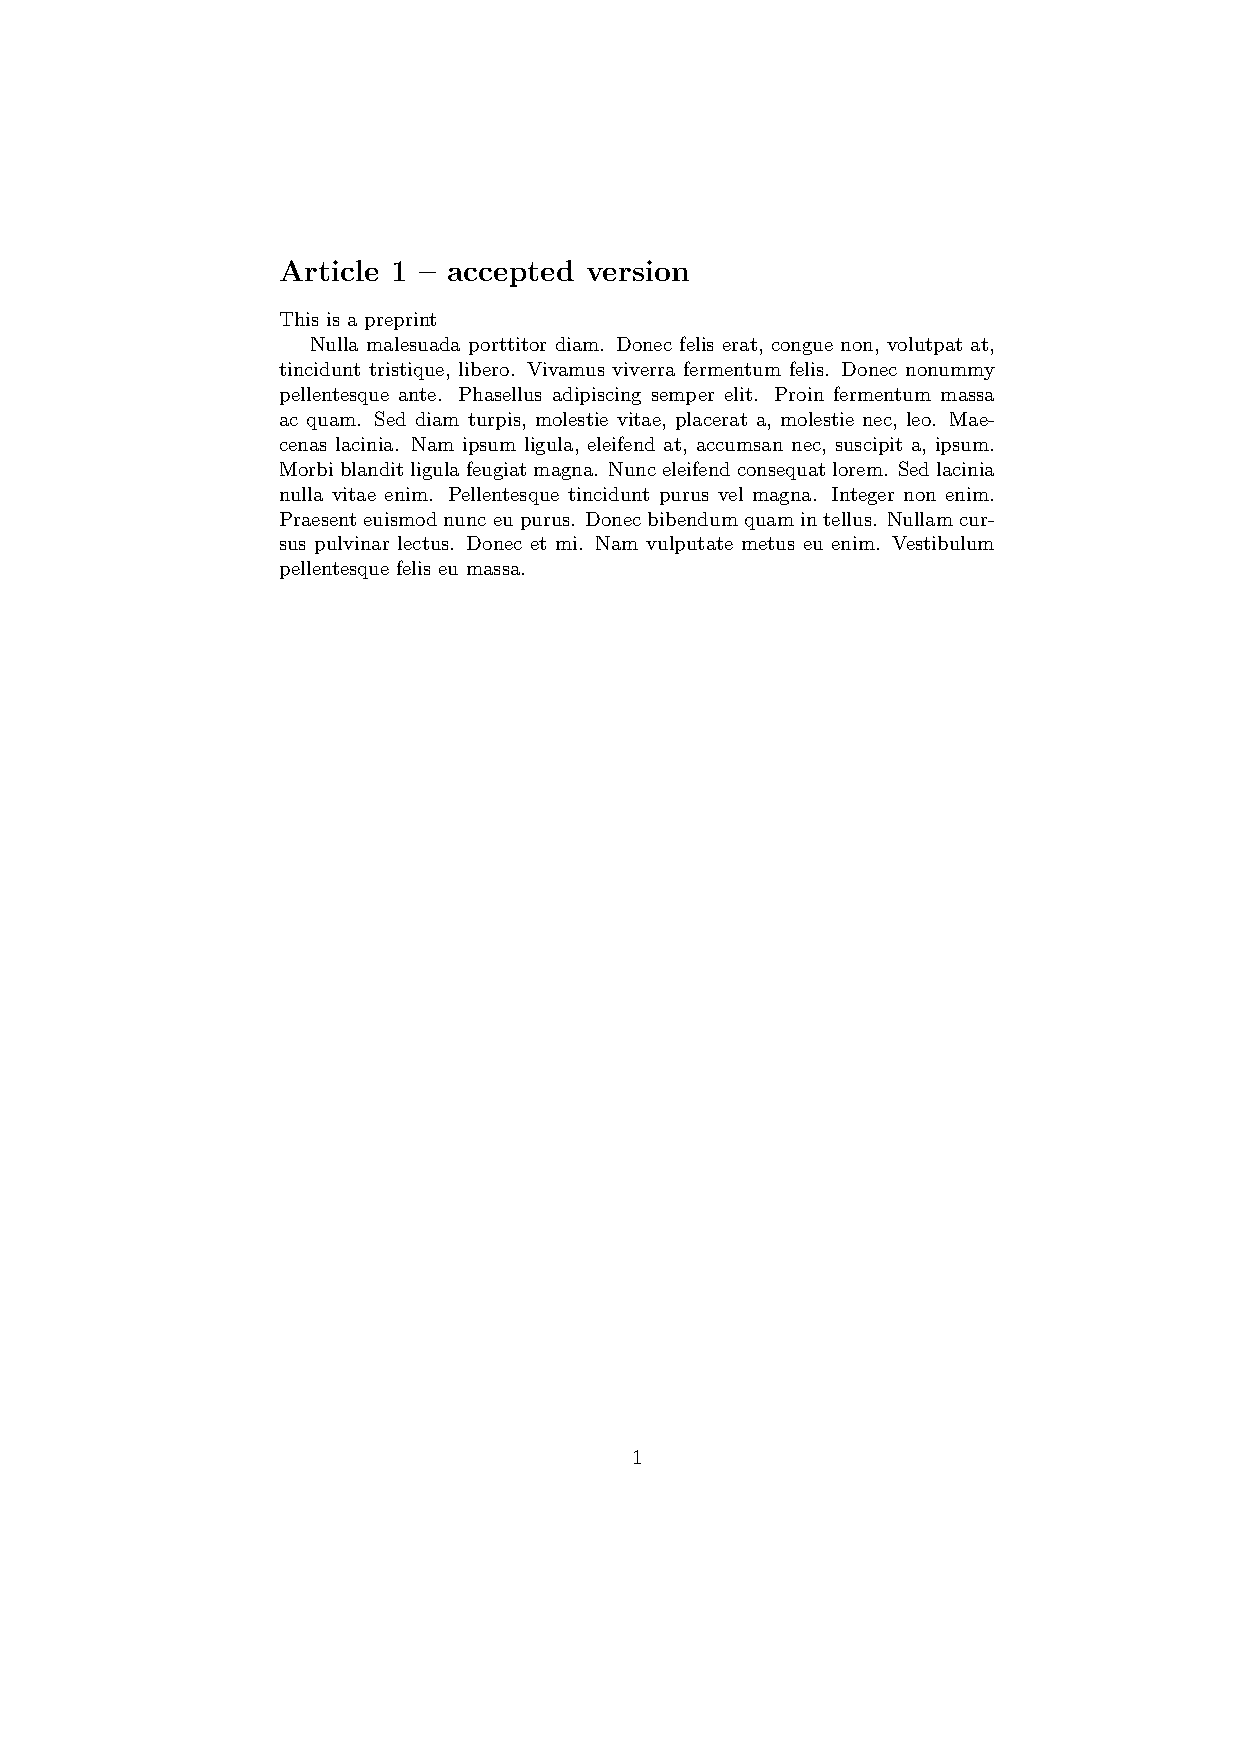
\includepdf[pages=1\allp, clip, trim=1cm 1cm 1cm 1cm]{articles/article1_accepted.pdf}
}{% Published (i.e. printed) version
    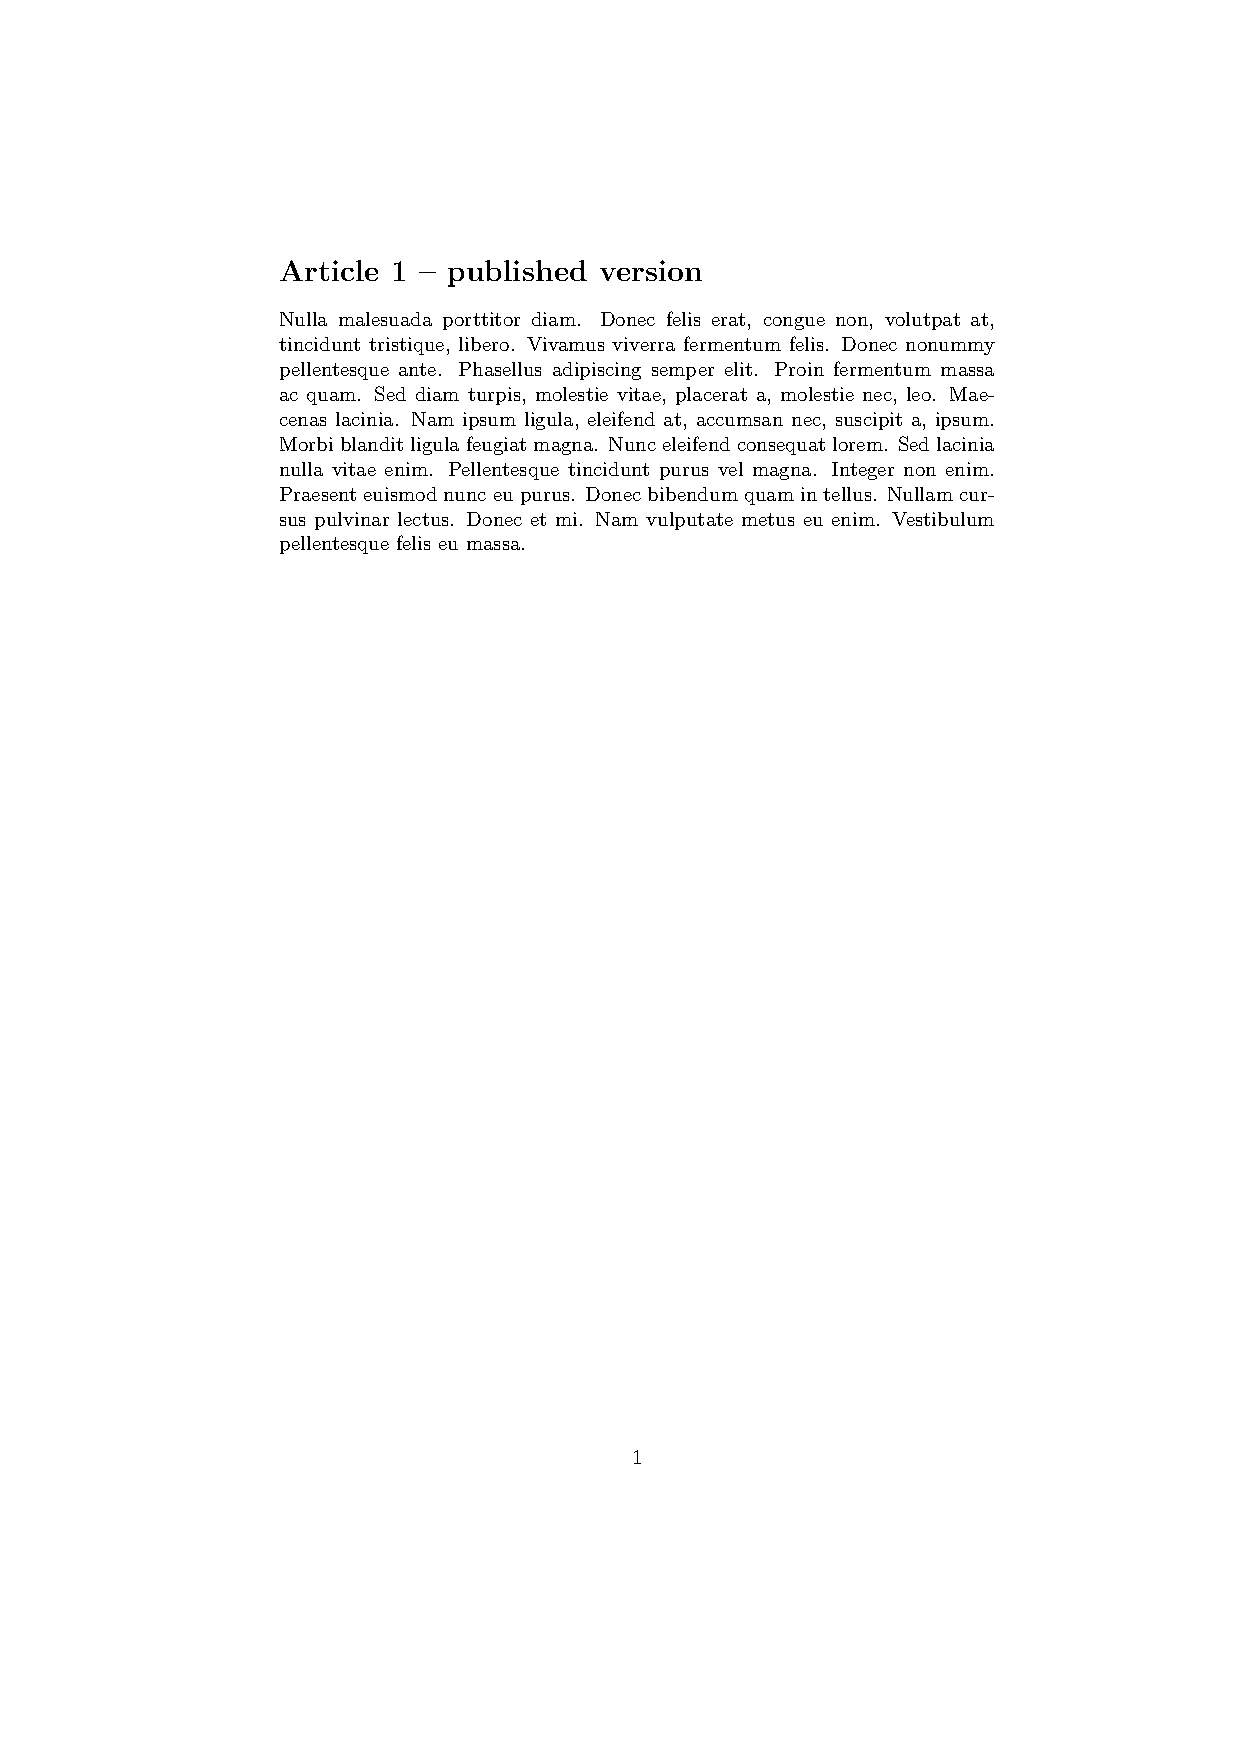
\includepdf[pages=1\allp, clip, trim=1cm 3cm 2cm 1cm]{articles/article1_published.pdf}
}{34} % Skip this many pages to keep numbering correct
\cleardoublepage


%%%%% %%%%% %%%%% %%%%% %%%%%


\begin{papertitle}{anotherArticle}{Another article}

    \ifOnlineVersion{\vfill The final authenticated version is available online at \href{https://doi.org/also-real-doi}{DOI:~also-real-doi}.}{}{0}\par
    
    The manuscript is reprinted with permission from Myself.
\end{papertitle}

\ifOnlineVersion{%
    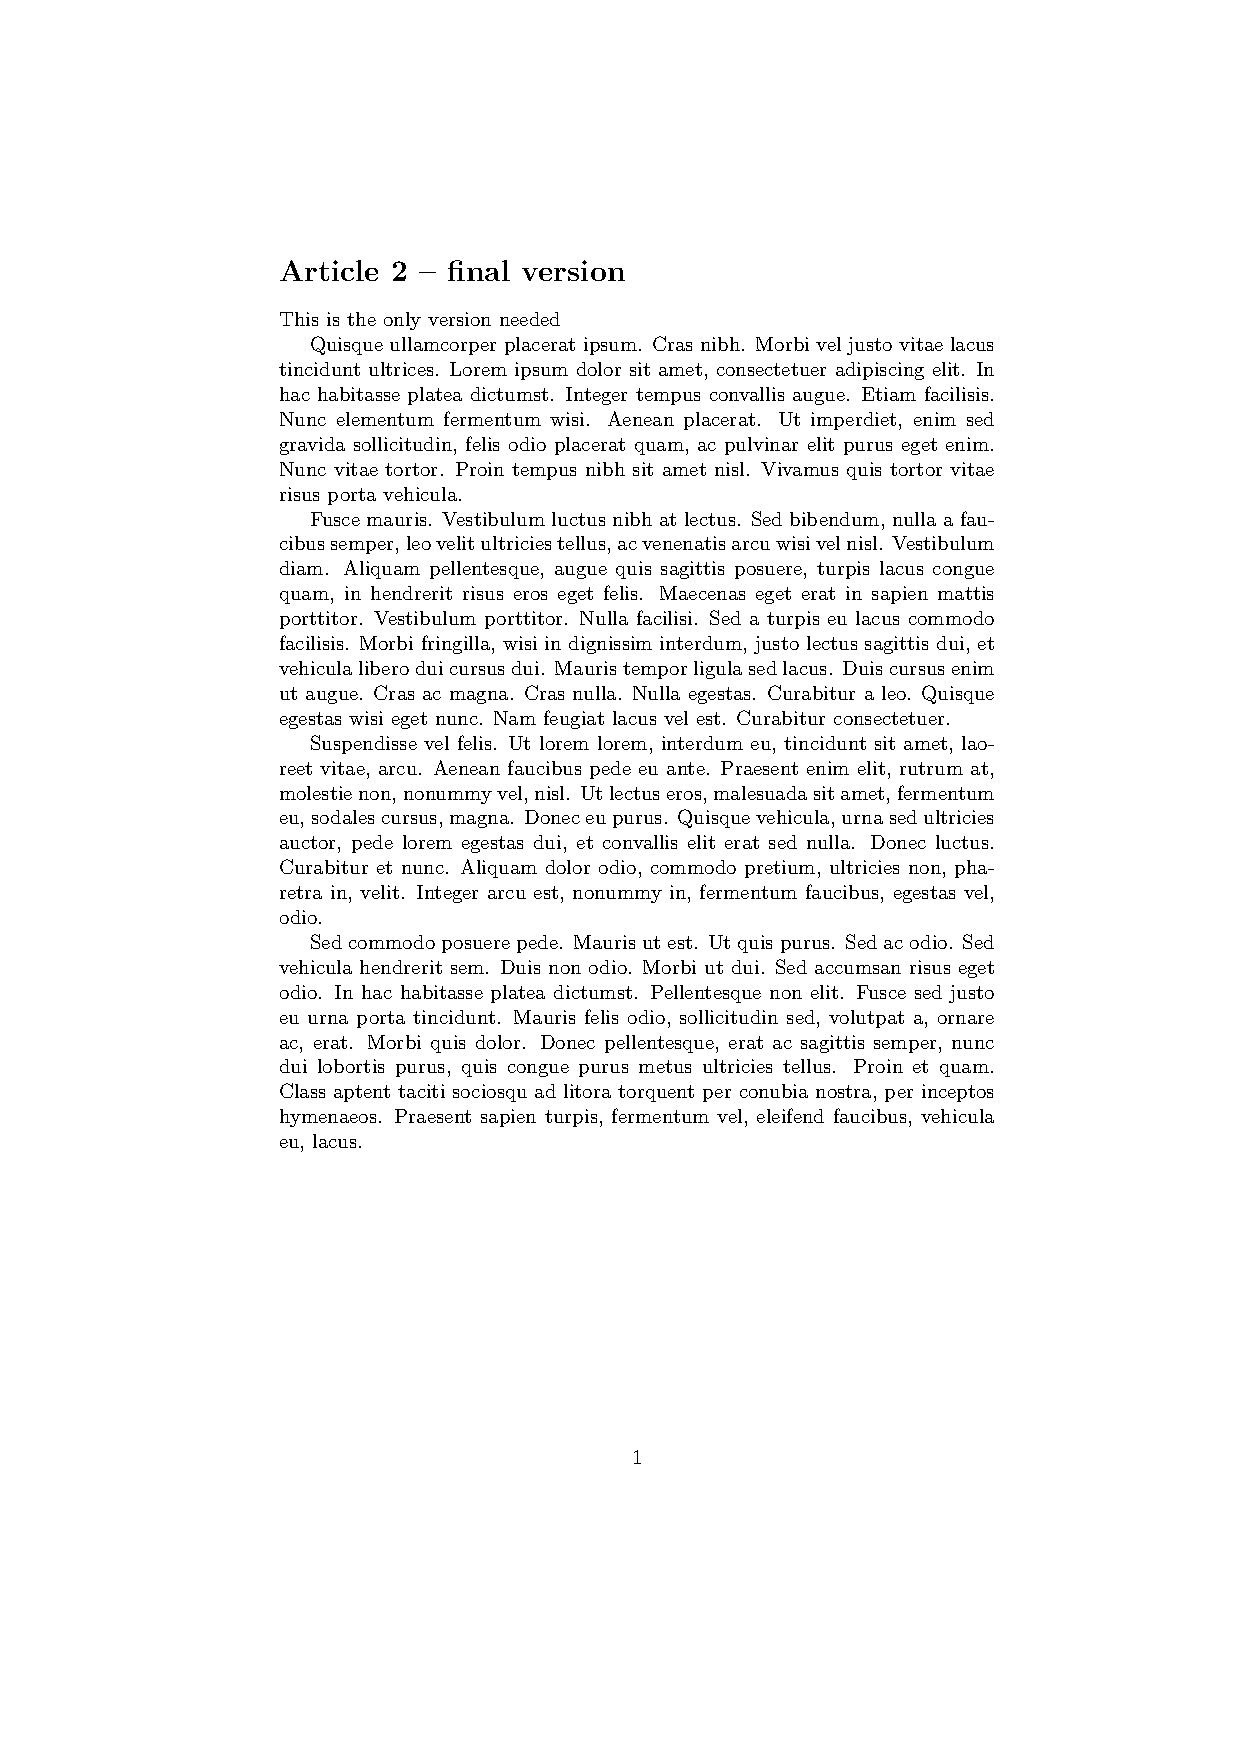
\includepdf[pages=1\allp, clip, trim=0cm 0cm 0cm 0cm]{articles/article2_final.pdf}
}{%
    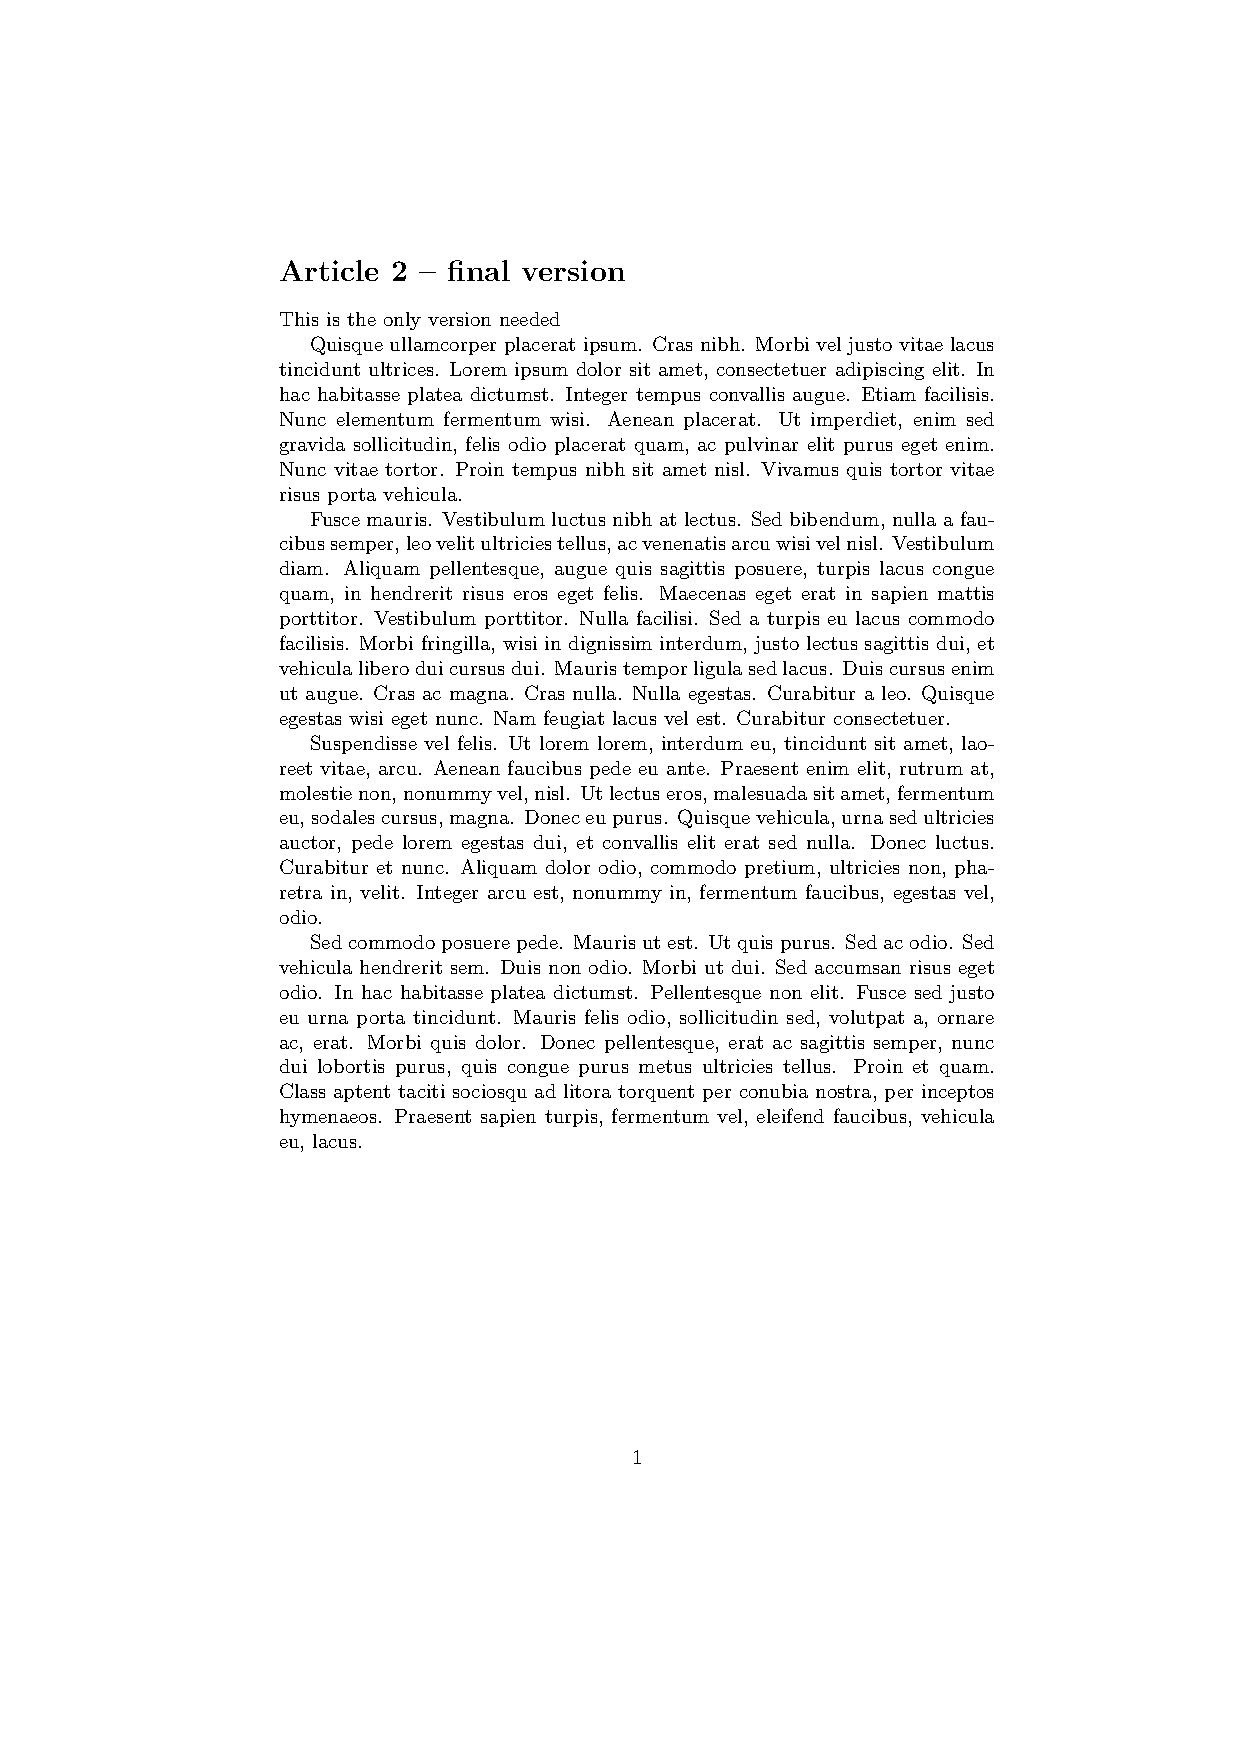
\includepdf[pages=1\allp, clip, trim=-0.2cm 0cm -0.2cm 0cm]{articles/article2_final.pdf}
}{11} % Skip this many pages to keep numbering correct
\cleardoublepage


%%%%% %%%%% %%%%% %%%%% %%%%%


\begin{comment}
\begin{papertitle}{thirdArticle}{The cool third article I could never finnish}
    \ifOnlineVersion{\vfill The final authenticated version is available online at \href{https://doi.org/10.1016/j.cam.2023.115206}{DOI:~10.1016/j.cam.2023.115206}.
    
    © 2023. This manuscript version is made available under the CC-BY-NC-ND 4.0 license \url{https://creativecommons.org/licenses/by-nc-nd/4.0/}.}{}{0}\par
    
    The manuscript is reprinted without permission.
\end{papertitle}
\ifOnlineVersion{%
    \includepdf[pages=1\allp, clip, trim=1cm 1cm 1cm 1cm]{articles/article3_accepted.pdf}
}{%
    \includepdf[pages=1\allp, clip, trim=-0.8cm 0cm -0.8cm 0cm]{articles/article3_published.pdf}
}{25}
\cleardoublepage
\end{comment}


%%%%% %%%%% %%%%% %%%%% %%%%%


\appendix

%%%%% Redefine chapter title style %%%%%
\titleformat
{\chapter} % command
[hang] % shape
{\vspace{-3cm}\bfseries \centering%
\rule{\textwidth-2cm}{0.5pt} \\
\rule{\textwidth-2cm}{1pt} \\[0.5em]} % format
{\LARGE Appendix \thechapter:} % label
{1em} % sep
{
\LARGE
} % before-code
[
\centering
\rule{\textwidth-2cm}{1pt} \\
\rule{\textwidth-2cm}{0.5pt} \\
\smallskip
]


%%%%% %%%%% %%%%% %%%%% %%%%%
%%%%%     APPENDIX      %%%%%
%%%%% %%%%% %%%%% %%%%% %%%%%

\pagestyle{plain}

      %%%%%       %%%%%       %%%%%       %%%%% 
%%%%%       %%%%%       %%%%%       %%%%%       %%%%%
\chapter{Algorithms} \label{ch:algorithms}
%%%%%       %%%%%       %%%%%       %%%%%       %%%%%
      %%%%%       %%%%%       %%%%%       %%%%% 

Here is the first appendix which contains an example algorithm. To simplify things, some macros are created first (but not rendered of course).

\newcommand{\fn}[1]{\texttt{#1}}
\newcommand{\fil}{\fn{filter}}
\newcommand{\fnsc}[1]{\textsc{#1}}

\section{First algorithm in appendix} \label{A:firstCode}

New things can still be cited, they will just appear in the biboliography which is printed already. We can also reference a specific line from the algorithm, like \cref{algline:LH}.

%%% Algorithm goes here!!! %%%
\begin{algorithm}[ht!]

\caption{2D discrete wavelet decomposition algorithm} \label{alg:waveletDec}

Here we can put some detailed explanation. For example this algorithm does
\begin{equation*}
    \W : \fvec \longmapsto (\vb{a}, \vb{d}_1, ..., \vb{d}_J),
\end{equation*}
which is great.

\begin{algorithmic}[1]
\Ensure real-valued array $\vb{f}[k_1,k_2]$ of size $n_1 \times n_2$, decomposition level $J$, low-pass filter $l[k]$, high-pass filter $h[k]$

\hspace{-3.5em}\Output detail coefficients $\vb{d} = [\vb{d}_1, \hdots, \vb{d}_J]$ for each scale, approximation coefficients $\vb{a}$ for coarsest scale
\Require $J \leqslant \log_2(\min\lbrace n_1, n_2 \rbrace )$
\State $n = \Call{length}{h}$ \Comment{We assume both filters have the same length}
\State $\vb{a} \gets \vb{f}$ \Comment{Initial input}
\For{scale $j = J:1$}

\BeginBox[dashed, draw=gray]
\State $\vb{a} \gets \Call{padData}{\vb{a}, n-1, \dim = 1}$ \Comment{Pad data based on filter length $n$}

\State $L \gets \Call{conv}{\vb{a}, l, \dim = 1}$
\State $H \gets \Call{conv}{\vb{a}, h, \dim = 1}$

\State $L \gets \Call{downsample}{L, \dim = 1}$
\State $H \gets \Call{downsample}{H, \dim = 1}$

\Statex % This creates an empty line
\State $L \gets \Call{padData}{L, n-1, \dim = 2}$
\State $H \gets \Call{padData}{H, n-1, \dim = 2}$

\State $LL \gets \Call{conv}{L, l, \dim = 2}$ \label{algline:LL}
\State $LH \gets \Call{conv}{L, h, \dim = 2}$ \label{algline:LH}
\State $HL \gets \Call{conv}{H, l, \dim = 2}$
\State $HH \gets \Call{conv}{H, h, \dim = 2}$

\State $\vb{a} \gets \Call{downsample}{LL, \dim = 2}$
\State $LH \gets \Call{downsample}{LH, \dim = 2}$
\State $HL \gets \Call{downsample}{HL, \dim = 2}$
\State $HH \gets \Call{downsample}{HH, \dim = 2}$
\EndBox
\State $\vb{d}_j \gets [LH, HL, HH]$
\EndFor

\State \Return{$[\vb{d}_1,\hdots, \vb{d}_J]$ and $\vb{a}$}
\end{algorithmic}
\end{algorithm}

\vfill

\end{document}
